\documentclass[11pt]{article}
    \usepackage[breakable]{tcolorbox}
    \usepackage{parskip} % Stop auto-indenting (to mimic markdown behaviour)
    \usepackage[utf8x]{inputenc}


    \usepackage{iftex}
    \ifPDFTeX
    	\usepackage[T1]{fontenc}
    	\usepackage{mathpazo}
    \else
    	\usepackage{fontspec}
    \fi

    % Basic figure setup, for now with no caption control since it's done
    % automatically by Pandoc (which extracts ![](path) syntax from Markdown).
    \usepackage{graphicx}
    % Maintain compatibility with old templates. Remove in nbconvert 6.0
    \let\Oldincludegraphics\includegraphics
    % Ensure that by default, figures have no caption (until we provide a
    % proper Figure object with a Caption API and a way to capture that
    % in the conversion process - todo).
    \usepackage{caption}
    \DeclareCaptionFormat{nocaption}{}
    \captionsetup{format=nocaption,aboveskip=0pt,belowskip=0pt}

    \usepackage{float}
    \floatplacement{figure}{H} % forces figures to be placed at the correct location
    \usepackage{xcolor} % Allow colors to be defined
    \usepackage{enumerate} % Needed for markdown enumerations to work
    \usepackage{geometry} % Used to adjust the document margins
    \usepackage{amsmath} % Equations
    \usepackage{amssymb} % Equations
    \usepackage{textcomp} % defines textquotesingle
    % Hack from http://tex.stackexchange.com/a/47451/13684:
    \AtBeginDocument{%
        \def\PYZsq{\textquotesingle}% Upright quotes in Pygmentized code
    }
    \usepackage{upquote} % Upright quotes for verbatim code
    \usepackage{eurosym} % defines \euro
    % \usepackage[mathletters]{ucs} % Extended unicode (utf-8) support
    \usepackage{fancyvrb} % verbatim replacement that allows latex
    \usepackage{grffile} % extends the file name processing of package graphics 
                         % to support a larger range
    \makeatletter % fix for old versions of grffile with XeLaTeX
    \@ifpackagelater{grffile}{2019/11/01}
    {
      % Do nothing on new versions
    }
    {
      \def\Gread@@xetex#1{%
        \IfFileExists{"\Gin@base".bb}%
        {\Gread@eps{\Gin@base.bb}}%
        {\Gread@@xetex@aux#1}%
      }
    }
    \makeatother
    \usepackage[Export]{adjustbox} % Used to constrain images to a maximum size
    \adjustboxset{max size={0.9\linewidth}{0.9\paperheight}}

    % The hyperref package gives us a pdf with properly built
    % internal navigation ('pdf bookmarks' for the table of contents,
    % internal cross-reference links, web links for URLs, etc.)
    \usepackage{hyperref}
    % The default LaTeX title has an obnoxious amount of whitespace. By default,
    % titling removes some of it. It also provides customization options.
    \usepackage{titling}
    \usepackage{longtable} % longtable support required by pandoc >1.10
    \usepackage{booktabs}  % table support for pandoc > 1.12.2
    \usepackage[inline]{enumitem} % IRkernel/repr support (it uses the enumerate* environment)
    \usepackage[normalem]{ulem} % ulem is needed to support strikethroughs (\sout)
                                % normalem makes italics be italics, not underlines
    \usepackage{mathrsfs}
    

    
    % Colors for the hyperref package
    \definecolor{urlcolor}{rgb}{0,.145,.698}
    \definecolor{linkcolor}{rgb}{.71,0.21,0.01}
    \definecolor{citecolor}{rgb}{.12,.54,.11}

    % ANSI colors
    \definecolor{ansi-black}{HTML}{3E424D}
    \definecolor{ansi-black-intense}{HTML}{282C36}
    \definecolor{ansi-red}{HTML}{E75C58}
    \definecolor{ansi-red-intense}{HTML}{B22B31}
    \definecolor{ansi-green}{HTML}{00A250}
    \definecolor{ansi-green-intense}{HTML}{007427}
    \definecolor{ansi-yellow}{HTML}{DDB62B}
    \definecolor{ansi-yellow-intense}{HTML}{B27D12}
    \definecolor{ansi-blue}{HTML}{208FFB}
    \definecolor{ansi-blue-intense}{HTML}{0065CA}
    \definecolor{ansi-magenta}{HTML}{D160C4}
    \definecolor{ansi-magenta-intense}{HTML}{A03196}
    \definecolor{ansi-cyan}{HTML}{60C6C8}
    \definecolor{ansi-cyan-intense}{HTML}{258F8F}
    \definecolor{ansi-white}{HTML}{C5C1B4}
    \definecolor{ansi-white-intense}{HTML}{A1A6B2}
    \definecolor{ansi-default-inverse-fg}{HTML}{FFFFFF}
    \definecolor{ansi-default-inverse-bg}{HTML}{000000}

    % common color for the border for error outputs.
    \definecolor{outerrorbackground}{HTML}{FFDFDF}

    % commands and environments needed by pandoc snippets
    % extracted from the output of `pandoc -s`
    \providecommand{\tightlist}{%
      \setlength{\itemsep}{0pt}\setlength{\parskip}{0pt}}
    \DefineVerbatimEnvironment{Highlighting}{Verbatim}{commandchars=\\\{\}}
    % Add ',fontsize=\small' for more characters per line
    \newenvironment{Shaded}{}{}
    \newcommand{\KeywordTok}[1]{\textcolor[rgb]{0.00,0.44,0.13}{\textbf{{#1}}}}
    \newcommand{\DataTypeTok}[1]{\textcolor[rgb]{0.56,0.13,0.00}{{#1}}}
    \newcommand{\DecValTok}[1]{\textcolor[rgb]{0.25,0.63,0.44}{{#1}}}
    \newcommand{\BaseNTok}[1]{\textcolor[rgb]{0.25,0.63,0.44}{{#1}}}
    \newcommand{\FloatTok}[1]{\textcolor[rgb]{0.25,0.63,0.44}{{#1}}}
    \newcommand{\CharTok}[1]{\textcolor[rgb]{0.25,0.44,0.63}{{#1}}}
    \newcommand{\StringTok}[1]{\textcolor[rgb]{0.25,0.44,0.63}{{#1}}}
    \newcommand{\CommentTok}[1]{\textcolor[rgb]{0.38,0.63,0.69}{\textit{{#1}}}}
    \newcommand{\OtherTok}[1]{\textcolor[rgb]{0.00,0.44,0.13}{{#1}}}
    \newcommand{\AlertTok}[1]{\textcolor[rgb]{1.00,0.00,0.00}{\textbf{{#1}}}}
    \newcommand{\FunctionTok}[1]{\textcolor[rgb]{0.02,0.16,0.49}{{#1}}}
    \newcommand{\RegionMarkerTok}[1]{{#1}}
    \newcommand{\ErrorTok}[1]{\textcolor[rgb]{1.00,0.00,0.00}{\textbf{{#1}}}}
    \newcommand{\NormalTok}[1]{{#1}}
    
    % Additional commands for more recent versions of Pandoc
    \newcommand{\ConstantTok}[1]{\textcolor[rgb]{0.53,0.00,0.00}{{#1}}}
    \newcommand{\SpecialCharTok}[1]{\textcolor[rgb]{0.25,0.44,0.63}{{#1}}}
    \newcommand{\VerbatimStringTok}[1]{\textcolor[rgb]{0.25,0.44,0.63}{{#1}}}
    \newcommand{\SpecialStringTok}[1]{\textcolor[rgb]{0.73,0.40,0.53}{{#1}}}
    \newcommand{\ImportTok}[1]{{#1}}
    \newcommand{\DocumentationTok}[1]{\textcolor[rgb]{0.73,0.13,0.13}{\textit{{#1}}}}
    \newcommand{\AnnotationTok}[1]{\textcolor[rgb]{0.38,0.63,0.69}{\textbf{\textit{{#1}}}}}
    \newcommand{\CommentVarTok}[1]{\textcolor[rgb]{0.38,0.63,0.69}{\textbf{\textit{{#1}}}}}
    \newcommand{\VariableTok}[1]{\textcolor[rgb]{0.10,0.09,0.49}{{#1}}}
    \newcommand{\ControlFlowTok}[1]{\textcolor[rgb]{0.00,0.44,0.13}{\textbf{{#1}}}}
    \newcommand{\OperatorTok}[1]{\textcolor[rgb]{0.40,0.40,0.40}{{#1}}}
    \newcommand{\BuiltInTok}[1]{{#1}}
    \newcommand{\ExtensionTok}[1]{{#1}}
    \newcommand{\PreprocessorTok}[1]{\textcolor[rgb]{0.74,0.48,0.00}{{#1}}}
    \newcommand{\AttributeTok}[1]{\textcolor[rgb]{0.49,0.56,0.16}{{#1}}}
    \newcommand{\InformationTok}[1]{\textcolor[rgb]{0.38,0.63,0.69}{\textbf{\textit{{#1}}}}}
    \newcommand{\WarningTok}[1]{\textcolor[rgb]{0.38,0.63,0.69}{\textbf{\textit{{#1}}}}}
    
    
    % Define a nice break command that doesn't care if a line doesn't already
    % exist.
    \def\br{\hspace*{\fill} \\* }
    % Math Jax compatibility definitions
    \def\gt{>}
    \def\lt{<}
    \let\Oldtex\TeX
    \let\Oldlatex\LaTeX
    \renewcommand{\TeX}{\textrm{\Oldtex}}
    \renewcommand{\LaTeX}{\textrm{\Oldlatex}}
    % Document parameters
    % Document title
    \title{Matplotlib Basics}
    \date{}
    
% Pygments definitions
\makeatletter
\def\PY@reset{\let\PY@it=\relax \let\PY@bf=\relax%
    \let\PY@ul=\relax \let\PY@tc=\relax%
    \let\PY@bc=\relax \let\PY@ff=\relax}
\def\PY@tok#1{\csname PY@tok@#1\endcsname}
\def\PY@toks#1+{\ifx\relax#1\empty\else%
    \PY@tok{#1}\expandafter\PY@toks\fi}
\def\PY@do#1{\PY@bc{\PY@tc{\PY@ul{%
    \PY@it{\PY@bf{\PY@ff{#1}}}}}}}
\def\PY#1#2{\PY@reset\PY@toks#1+\relax+\PY@do{#2}}

\@namedef{PY@tok@w}{\def\PY@tc##1{\textcolor[rgb]{0.73,0.73,0.73}{##1}}}
\@namedef{PY@tok@c}{\let\PY@it=\textit\def\PY@tc##1{\textcolor[rgb]{0.25,0.50,0.50}{##1}}}
\@namedef{PY@tok@cp}{\def\PY@tc##1{\textcolor[rgb]{0.74,0.48,0.00}{##1}}}
\@namedef{PY@tok@k}{\let\PY@bf=\textbf\def\PY@tc##1{\textcolor[rgb]{0.00,0.50,0.00}{##1}}}
\@namedef{PY@tok@kp}{\def\PY@tc##1{\textcolor[rgb]{0.00,0.50,0.00}{##1}}}
\@namedef{PY@tok@kt}{\def\PY@tc##1{\textcolor[rgb]{0.69,0.00,0.25}{##1}}}
\@namedef{PY@tok@o}{\def\PY@tc##1{\textcolor[rgb]{0.40,0.40,0.40}{##1}}}
\@namedef{PY@tok@ow}{\let\PY@bf=\textbf\def\PY@tc##1{\textcolor[rgb]{0.67,0.13,1.00}{##1}}}
\@namedef{PY@tok@nb}{\def\PY@tc##1{\textcolor[rgb]{0.00,0.50,0.00}{##1}}}
\@namedef{PY@tok@nf}{\def\PY@tc##1{\textcolor[rgb]{0.00,0.00,1.00}{##1}}}
\@namedef{PY@tok@nc}{\let\PY@bf=\textbf\def\PY@tc##1{\textcolor[rgb]{0.00,0.00,1.00}{##1}}}
\@namedef{PY@tok@nn}{\let\PY@bf=\textbf\def\PY@tc##1{\textcolor[rgb]{0.00,0.00,1.00}{##1}}}
\@namedef{PY@tok@ne}{\let\PY@bf=\textbf\def\PY@tc##1{\textcolor[rgb]{0.82,0.25,0.23}{##1}}}
\@namedef{PY@tok@nv}{\def\PY@tc##1{\textcolor[rgb]{0.10,0.09,0.49}{##1}}}
\@namedef{PY@tok@no}{\def\PY@tc##1{\textcolor[rgb]{0.53,0.00,0.00}{##1}}}
\@namedef{PY@tok@nl}{\def\PY@tc##1{\textcolor[rgb]{0.63,0.63,0.00}{##1}}}
\@namedef{PY@tok@ni}{\let\PY@bf=\textbf\def\PY@tc##1{\textcolor[rgb]{0.60,0.60,0.60}{##1}}}
\@namedef{PY@tok@na}{\def\PY@tc##1{\textcolor[rgb]{0.49,0.56,0.16}{##1}}}
\@namedef{PY@tok@nt}{\let\PY@bf=\textbf\def\PY@tc##1{\textcolor[rgb]{0.00,0.50,0.00}{##1}}}
\@namedef{PY@tok@nd}{\def\PY@tc##1{\textcolor[rgb]{0.67,0.13,1.00}{##1}}}
\@namedef{PY@tok@s}{\def\PY@tc##1{\textcolor[rgb]{0.73,0.13,0.13}{##1}}}
\@namedef{PY@tok@sd}{\let\PY@it=\textit\def\PY@tc##1{\textcolor[rgb]{0.73,0.13,0.13}{##1}}}
\@namedef{PY@tok@si}{\let\PY@bf=\textbf\def\PY@tc##1{\textcolor[rgb]{0.73,0.40,0.53}{##1}}}
\@namedef{PY@tok@se}{\let\PY@bf=\textbf\def\PY@tc##1{\textcolor[rgb]{0.73,0.40,0.13}{##1}}}
\@namedef{PY@tok@sr}{\def\PY@tc##1{\textcolor[rgb]{0.73,0.40,0.53}{##1}}}
\@namedef{PY@tok@ss}{\def\PY@tc##1{\textcolor[rgb]{0.10,0.09,0.49}{##1}}}
\@namedef{PY@tok@sx}{\def\PY@tc##1{\textcolor[rgb]{0.00,0.50,0.00}{##1}}}
\@namedef{PY@tok@m}{\def\PY@tc##1{\textcolor[rgb]{0.40,0.40,0.40}{##1}}}
\@namedef{PY@tok@gh}{\let\PY@bf=\textbf\def\PY@tc##1{\textcolor[rgb]{0.00,0.00,0.50}{##1}}}
\@namedef{PY@tok@gu}{\let\PY@bf=\textbf\def\PY@tc##1{\textcolor[rgb]{0.50,0.00,0.50}{##1}}}
\@namedef{PY@tok@gd}{\def\PY@tc##1{\textcolor[rgb]{0.63,0.00,0.00}{##1}}}
\@namedef{PY@tok@gi}{\def\PY@tc##1{\textcolor[rgb]{0.00,0.63,0.00}{##1}}}
\@namedef{PY@tok@gr}{\def\PY@tc##1{\textcolor[rgb]{1.00,0.00,0.00}{##1}}}
\@namedef{PY@tok@ge}{\let\PY@it=\textit}
\@namedef{PY@tok@gs}{\let\PY@bf=\textbf}
\@namedef{PY@tok@gp}{\let\PY@bf=\textbf\def\PY@tc##1{\textcolor[rgb]{0.00,0.00,0.50}{##1}}}
\@namedef{PY@tok@go}{\def\PY@tc##1{\textcolor[rgb]{0.53,0.53,0.53}{##1}}}
\@namedef{PY@tok@gt}{\def\PY@tc##1{\textcolor[rgb]{0.00,0.27,0.87}{##1}}}
\@namedef{PY@tok@err}{\def\PY@bc##1{{\setlength{\fboxsep}{\string -\fboxrule}\fcolorbox[rgb]{1.00,0.00,0.00}{1,1,1}{\strut ##1}}}}
\@namedef{PY@tok@kc}{\let\PY@bf=\textbf\def\PY@tc##1{\textcolor[rgb]{0.00,0.50,0.00}{##1}}}
\@namedef{PY@tok@kd}{\let\PY@bf=\textbf\def\PY@tc##1{\textcolor[rgb]{0.00,0.50,0.00}{##1}}}
\@namedef{PY@tok@kn}{\let\PY@bf=\textbf\def\PY@tc##1{\textcolor[rgb]{0.00,0.50,0.00}{##1}}}
\@namedef{PY@tok@kr}{\let\PY@bf=\textbf\def\PY@tc##1{\textcolor[rgb]{0.00,0.50,0.00}{##1}}}
\@namedef{PY@tok@bp}{\def\PY@tc##1{\textcolor[rgb]{0.00,0.50,0.00}{##1}}}
\@namedef{PY@tok@fm}{\def\PY@tc##1{\textcolor[rgb]{0.00,0.00,1.00}{##1}}}
\@namedef{PY@tok@vc}{\def\PY@tc##1{\textcolor[rgb]{0.10,0.09,0.49}{##1}}}
\@namedef{PY@tok@vg}{\def\PY@tc##1{\textcolor[rgb]{0.10,0.09,0.49}{##1}}}
\@namedef{PY@tok@vi}{\def\PY@tc##1{\textcolor[rgb]{0.10,0.09,0.49}{##1}}}
\@namedef{PY@tok@vm}{\def\PY@tc##1{\textcolor[rgb]{0.10,0.09,0.49}{##1}}}
\@namedef{PY@tok@sa}{\def\PY@tc##1{\textcolor[rgb]{0.73,0.13,0.13}{##1}}}
\@namedef{PY@tok@sb}{\def\PY@tc##1{\textcolor[rgb]{0.73,0.13,0.13}{##1}}}
\@namedef{PY@tok@sc}{\def\PY@tc##1{\textcolor[rgb]{0.73,0.13,0.13}{##1}}}
\@namedef{PY@tok@dl}{\def\PY@tc##1{\textcolor[rgb]{0.73,0.13,0.13}{##1}}}
\@namedef{PY@tok@s2}{\def\PY@tc##1{\textcolor[rgb]{0.73,0.13,0.13}{##1}}}
\@namedef{PY@tok@sh}{\def\PY@tc##1{\textcolor[rgb]{0.73,0.13,0.13}{##1}}}
\@namedef{PY@tok@s1}{\def\PY@tc##1{\textcolor[rgb]{0.73,0.13,0.13}{##1}}}
\@namedef{PY@tok@mb}{\def\PY@tc##1{\textcolor[rgb]{0.40,0.40,0.40}{##1}}}
\@namedef{PY@tok@mf}{\def\PY@tc##1{\textcolor[rgb]{0.40,0.40,0.40}{##1}}}
\@namedef{PY@tok@mh}{\def\PY@tc##1{\textcolor[rgb]{0.40,0.40,0.40}{##1}}}
\@namedef{PY@tok@mi}{\def\PY@tc##1{\textcolor[rgb]{0.40,0.40,0.40}{##1}}}
\@namedef{PY@tok@il}{\def\PY@tc##1{\textcolor[rgb]{0.40,0.40,0.40}{##1}}}
\@namedef{PY@tok@mo}{\def\PY@tc##1{\textcolor[rgb]{0.40,0.40,0.40}{##1}}}
\@namedef{PY@tok@ch}{\let\PY@it=\textit\def\PY@tc##1{\textcolor[rgb]{0.25,0.50,0.50}{##1}}}
\@namedef{PY@tok@cm}{\let\PY@it=\textit\def\PY@tc##1{\textcolor[rgb]{0.25,0.50,0.50}{##1}}}
\@namedef{PY@tok@cpf}{\let\PY@it=\textit\def\PY@tc##1{\textcolor[rgb]{0.25,0.50,0.50}{##1}}}
\@namedef{PY@tok@c1}{\let\PY@it=\textit\def\PY@tc##1{\textcolor[rgb]{0.25,0.50,0.50}{##1}}}
\@namedef{PY@tok@cs}{\let\PY@it=\textit\def\PY@tc##1{\textcolor[rgb]{0.25,0.50,0.50}{##1}}}

\def\PYZbs{\char`\\}
\def\PYZus{\char`\_}
\def\PYZob{\char`\{}
\def\PYZcb{\char`\}}
\def\PYZca{\char`\^}
\def\PYZam{\char`\&}
\def\PYZlt{\char`\<}
\def\PYZgt{\char`\>}
\def\PYZsh{\char`\#}
\def\PYZpc{\char`\%}
\def\PYZdl{\char`\$}
\def\PYZhy{\char`\-}
\def\PYZsq{\char`\'}
\def\PYZdq{\char`\"}
\def\PYZti{\char`\~}
% for compatibility with earlier versions
\def\PYZat{@}
\def\PYZlb{[}
\def\PYZrb{]}
\makeatother


    % For linebreaks inside Verbatim environment from package fancyvrb. 
    \makeatletter
        \newbox\Wrappedcontinuationbox 
        \newbox\Wrappedvisiblespacebox 
        \newcommand*\Wrappedvisiblespace {\textcolor{red}{\textvisiblespace}} 
        \newcommand*\Wrappedcontinuationsymbol {\textcolor{red}{\llap{\tiny$\m@th\hookrightarrow$}}} 
        \newcommand*\Wrappedcontinuationindent {3ex } 
        \newcommand*\Wrappedafterbreak {\kern\Wrappedcontinuationindent\copy\Wrappedcontinuationbox} 
        % Take advantage of the already applied Pygments mark-up to insert 
        % potential linebreaks for TeX processing. 
        %        {, <, #, %, $, ' and ": go to next line. 
        %        _, }, ^, &, >, - and ~: stay at end of broken line. 
        % Use of \textquotesingle for straight quote. 
        \newcommand*\Wrappedbreaksatspecials {% 
            \def\PYGZus{\discretionary{\char`\_}{\Wrappedafterbreak}{\char`\_}}% 
            \def\PYGZob{\discretionary{}{\Wrappedafterbreak\char`\{}{\char`\{}}% 
            \def\PYGZcb{\discretionary{\char`\}}{\Wrappedafterbreak}{\char`\}}}% 
            \def\PYGZca{\discretionary{\char`\^}{\Wrappedafterbreak}{\char`\^}}% 
            \def\PYGZam{\discretionary{\char`\&}{\Wrappedafterbreak}{\char`\&}}% 
            \def\PYGZlt{\discretionary{}{\Wrappedafterbreak\char`\<}{\char`\<}}% 
            \def\PYGZgt{\discretionary{\char`\>}{\Wrappedafterbreak}{\char`\>}}% 
            \def\PYGZsh{\discretionary{}{\Wrappedafterbreak\char`\#}{\char`\#}}% 
            \def\PYGZpc{\discretionary{}{\Wrappedafterbreak\char`\%}{\char`\%}}% 
            \def\PYGZdl{\discretionary{}{\Wrappedafterbreak\char`\$}{\char`\$}}% 
            \def\PYGZhy{\discretionary{\char`\-}{\Wrappedafterbreak}{\char`\-}}% 
            \def\PYGZsq{\discretionary{}{\Wrappedafterbreak\textquotesingle}{\textquotesingle}}% 
            \def\PYGZdq{\discretionary{}{\Wrappedafterbreak\char`\"}{\char`\"}}% 
            \def\PYGZti{\discretionary{\char`\~}{\Wrappedafterbreak}{\char`\~}}% 
        } 
        % Some characters . , ; ? ! / are not pygmentized. 
        % This macro makes them "active" and they will insert potential linebreaks 
        \newcommand*\Wrappedbreaksatpunct {% 
            \lccode`\~`\.\lowercase{\def~}{\discretionary{\hbox{\char`\.}}{\Wrappedafterbreak}{\hbox{\char`\.}}}% 
            \lccode`\~`\,\lowercase{\def~}{\discretionary{\hbox{\char`\,}}{\Wrappedafterbreak}{\hbox{\char`\,}}}% 
            \lccode`\~`\;\lowercase{\def~}{\discretionary{\hbox{\char`\;}}{\Wrappedafterbreak}{\hbox{\char`\;}}}% 
            \lccode`\~`\:\lowercase{\def~}{\discretionary{\hbox{\char`\:}}{\Wrappedafterbreak}{\hbox{\char`\:}}}% 
            \lccode`\~`\?\lowercase{\def~}{\discretionary{\hbox{\char`\?}}{\Wrappedafterbreak}{\hbox{\char`\?}}}% 
            \lccode`\~`\!\lowercase{\def~}{\discretionary{\hbox{\char`\!}}{\Wrappedafterbreak}{\hbox{\char`\!}}}% 
            \lccode`\~`\/\lowercase{\def~}{\discretionary{\hbox{\char`\/}}{\Wrappedafterbreak}{\hbox{\char`\/}}}% 
            \catcode`\.\active
            \catcode`\,\active 
            \catcode`\;\active
            \catcode`\:\active
            \catcode`\?\active
            \catcode`\!\active
            \catcode`\/\active 
            \lccode`\~`\~ 	
        }
    \makeatother

    \let\OriginalVerbatim=\Verbatim
    \makeatletter
    \renewcommand{\Verbatim}[1][1]{%
        %\parskip\z@skip
        \sbox\Wrappedcontinuationbox {\Wrappedcontinuationsymbol}%
        \sbox\Wrappedvisiblespacebox {\FV@SetupFont\Wrappedvisiblespace}%
        \def\FancyVerbFormatLine ##1{\hsize\linewidth
            \vtop{\raggedright\hyphenpenalty\z@\exhyphenpenalty\z@
                \doublehyphendemerits\z@\finalhyphendemerits\z@
                \strut ##1\strut}%
        }%
        % If the linebreak is at a space, the latter will be displayed as visible
        % space at end of first line, and a continuation symbol starts next line.
        % Stretch/shrink are however usually zero for typewriter font.
        \def\FV@Space {%
            \nobreak\hskip\z@ plus\fontdimen3\font minus\fontdimen4\font
            \discretionary{\copy\Wrappedvisiblespacebox}{\Wrappedafterbreak}
            {\kern\fontdimen2\font}%
        }%
        
        % Allow breaks at special characters using \PYG... macros.
        \Wrappedbreaksatspecials
        % Breaks at punctuation characters . , ; ? ! and / need catcode=\active 	
        \OriginalVerbatim[#1,codes*=\Wrappedbreaksatpunct]%
    }
    \makeatother

    % Exact colors from NB
    \definecolor{incolor}{HTML}{303F9F}
    \definecolor{outcolor}{HTML}{D84315}
    \definecolor{cellborder}{HTML}{CFCFCF}
    \definecolor{cellbackground}{HTML}{F7F7F7}
    
    % prompt
    \makeatletter
    \newcommand{\boxspacing}{\kern\kvtcb@left@rule\kern\kvtcb@boxsep}
    \makeatother
    \newcommand{\prompt}[4]{
        {\ttfamily\llap{{\color{#2}[#3]:\hspace{3pt}#4}}\vspace{-\baselineskip}}
    }
    

    
    % Prevent overflowing lines due to hard-to-break entities
    \sloppy 
    % Setup hyperref package
    \hypersetup{
      breaklinks=true,  % so long urls are correctly broken across lines
      colorlinks=true,
      urlcolor=urlcolor,
      linkcolor=linkcolor,
      citecolor=citecolor,
      }
    % Slightly bigger margins than the latex defaults
    
    \geometry{verbose,tmargin=2cm,bmargin=2cm,lmargin=2cm,rmargin=2cm}
    
    

\begin{document}
    
    \maketitle
    \vspace*{-1cm}
    \hypertarget{whats-matplotlib}{%
\section{What's Matplotlib?}\label{whats-matplotlib}}

Matplotlib is a popular data visualization library in Python. It allows
you to create a wide range of plots, such as line plots, scatter plots,
bar plots, histograms, and more.

\hypertarget{how-to-import-matplotlib}{%
\subsection{How to import
Matplotlib}\label{how-to-import-matplotlib}}

You can import Matplotlib using the following command:

\begin{Shaded}
\begin{Highlighting}[]
\ImportTok{import}\NormalTok{ matplotlib.pyplot }\ImportTok{as}\NormalTok{ plt}
\CommentTok{\# or from matplotlib import pyplot as plt}
\end{Highlighting}
\end{Shaded}

This is the standard way to import the library and gives you access to
the pyplot submodule, which provides a convenient interface for creating
and customizing plots.

\hypertarget{Figure-anatomy-in-matplotlib}{%
\subsection{Figure anatomy in matplotlib }\label{Figure-anatomy-in-matplotlib}}
The Matplotlib library, a Python library used for visualizing data, is built upon Numpy
and consists of a tree-like hierarchical structure composed of objects
that form each of the plots.

In Matplotlib, a ``Figure'' is the top-level container for a graph and
can contain multiple ``Axes'' objects, which are not to be confused with
the plural form of ``Axis''. An ``Axes'' object is a subplot that
resides within a ``Figure'' and can be used to manipulate every aspect
of the graph within it.

At the next level of the hierarchy beneath ``Axes'' are the tick marks,
lines, legends, and text boxes. Every object within Matplotlib can be
manipulated to create customized plots.

\begin{figure}
\centering
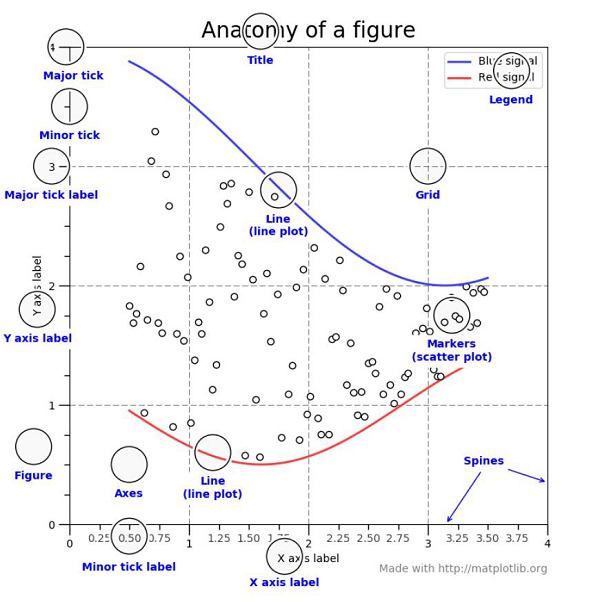
\includegraphics[scale=0.5]{fig_ana.jpg}
\end{figure}

\hypertarget{basic-plotting}{%
\section{Basic Plotting}\label{basic-plotting}}

In this section, we'll cover the foundational concepts of plotting with
Matplotlib.

\hypertarget{line-plots-and-scatter-plots}{%
\subsection{Line plots and Scatter
Plots}\label{line-plots-and-scatter-plots}}

\hypertarget{line-plots}{%
\paragraph{Line plots}\label{line-plots}}

To create a basic plot in Matplotlib, we can use the \texttt{plt.plot()}
function. This function generates a two-dimensional plot for one or more
iterable objects (lists of numbers or NumPy arrays) of points with known
x and y coordinates.

It is important to note that the length of the x and y objects should be
equal for the function to work correctly. For example, to plot the
\texttt{sin} function we use the following code:

\begin{Shaded}
\begin{Highlighting}[]
\ImportTok{import}\NormalTok{ matplotlib.pyplot }\ImportTok{as}\NormalTok{ plt}
\ImportTok{import}\NormalTok{ numpy }\ImportTok{as}\NormalTok{ np}
\CommentTok{\# Create an array of x values from 0 to 2*pi with a step size of 0.1}
\NormalTok{x }\OperatorTok{=}\NormalTok{ np.linspace(}\OperatorTok{{-}}\DecValTok{2}\OperatorTok{*}\NormalTok{np.pi, }\DecValTok{2}\OperatorTok{*}\NormalTok{np.pi, }\DecValTok{100}\NormalTok{)}

\CommentTok{\# Calculate y values for the sin function}
\NormalTok{y }\OperatorTok{=}\NormalTok{ np.sin(x)}

\CommentTok{\# Plot the sine function}
\NormalTok{plt.plot(x, y)}
\CommentTok{\# Diplay the result}
\NormalTok{plt.show()}
\end{Highlighting}
\end{Shaded}

\texttt{plt.plot} creates a Matplotlib object (here, a Line2D object)
and \texttt{plt.show()} displays it on the screen.

\begin{figure}
\centering
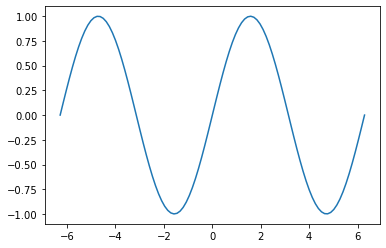
\includegraphics[scale=0.6]{plot.png}
\end{figure}

\hypertarget{scatter-plots}{%
\paragraph{Scatter plots}\label{scatter-plots}}

A scatter plot is a plot that shows the relationship between two
variables. Unlike other plots, it represents each data point as a dot
without any lines between them, with the position of the dot on the x
and y axes indicating the values of the two variables for that data
point. In Python, scatter plots can be created using
\texttt{plt.scatter()} function. For example, we can plot the scatter
plot of the previous function using the code: ```python import
matplotlib.pyplot as plt import numpy as np \# Create an array of x
values from 0 to 2\emph{pi with a step size of 0.1 x =
np.linspace(-2}np.pi, 2*np.pi, 100)

\hypertarget{calculate-y-values-for-the-sin-function}{%
\section{Calculate y values for the sin
function}\label{calculate-y-values-for-the-sin-function}}

y = np.sin(x)

\hypertarget{plot-the-sine-function}{%
\section{Plot the sine function}\label{plot-the-sine-function}}

plt.scatter(x, y) \# Diplay the result plt.show() ```

\begin{figure}
\centering
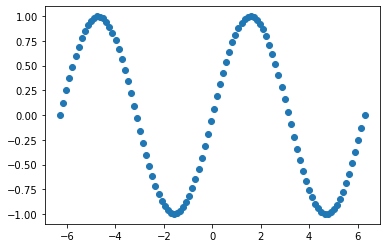
\includegraphics[scale=0.6]{scatter.png}
\end{figure}

\hypertarget{use-multiple-subplots-axes}{%
\section{Use multiple subplots
(axes)}\label{use-multiple-subplots-axes}}

You can create a new figure by calling the \texttt{plt.figure()}
function. Once you have created a figure, you can add one or more axes
objects to it using the \texttt{Figure.add\_subplot()} or
\texttt{plt.subplot()} methods which creates a grid of subplots within
the figure.

For example, to create a figure with a size of 8x6 inches contains a 2x2
grid of 4 subplots, you can use the following code:

\begin{Shaded}
\begin{Highlighting}[]
\ImportTok{import}\NormalTok{ matplotlib.pyplot }\ImportTok{as}\NormalTok{ plt}
\ImportTok{import}\NormalTok{ numpy }\ImportTok{as}\NormalTok{ np}
\NormalTok{fig}\OperatorTok{=}\NormalTok{plt.figure(figsize}\OperatorTok{=}\NormalTok{(}\DecValTok{8}\NormalTok{,}\DecValTok{6}\NormalTok{))}
\NormalTok{x}\OperatorTok{=}\NormalTok{np.linspace(}\OperatorTok{{-}}\DecValTok{10}\NormalTok{,}\DecValTok{10}\NormalTok{,}\DecValTok{100}\NormalTok{)}

\NormalTok{ax1 }\OperatorTok{=}\NormalTok{ fig.add\_subplot(}\DecValTok{3}\NormalTok{, }\DecValTok{2}\NormalTok{, }\DecValTok{1}\NormalTok{)}
\NormalTok{ax2 }\OperatorTok{=}\NormalTok{ fig.add\_subplot(}\DecValTok{3}\NormalTok{, }\DecValTok{2}\NormalTok{, }\DecValTok{2}\NormalTok{)}
\NormalTok{ax3 }\OperatorTok{=}\NormalTok{ fig.add\_subplot(}\DecValTok{3}\NormalTok{, }\DecValTok{2}\NormalTok{, }\DecValTok{3}\NormalTok{)}
\NormalTok{ax4 }\OperatorTok{=}\NormalTok{ fig.add\_subplot(}\DecValTok{3}\NormalTok{, }\DecValTok{2}\NormalTok{, }\DecValTok{4}\NormalTok{)}


\NormalTok{ax1.plot(x,np.power(x,}\FloatTok{1.}\NormalTok{)}\OperatorTok{*}\NormalTok{np.sin(x))}
\NormalTok{ax2.plot(x,np.power(x,}\FloatTok{2.}\NormalTok{)}\OperatorTok{*}\NormalTok{np.sin(x))}
\NormalTok{ax3.plot(x,np.power(x,}\FloatTok{3.}\NormalTok{)}\OperatorTok{*}\NormalTok{np.sin(x))}
\NormalTok{ax4.plot(x,np.power(x,}\FloatTok{4.}\NormalTok{)}\OperatorTok{*}\NormalTok{np.sin(x))}
\NormalTok{plt.show()}
\end{Highlighting}
\end{Shaded}

\begin{figure}
\centering
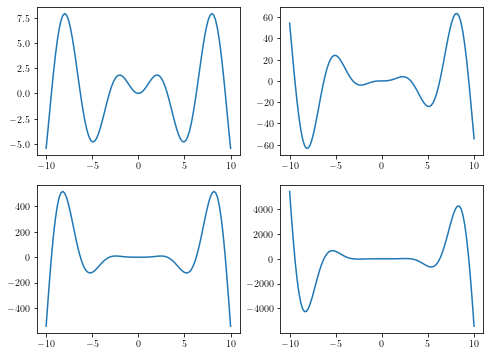
\includegraphics[scale=0.6]{addsubplot.png}
\end{figure}

\hypertarget{labels-legends-and-customization}{%
\section{Labels, Legends and
Customization}\label{labels-legends-and-customization}}

\hypertarget{labels-and-legends}{%
\subsection{Labels and Legends}\label{labels-and-legends}}

Labels and Legends are important components of a plot in Matplotlib that
help in providing information about the data presented in the plot.

\hypertarget{Plot-legend}{%
\subsubsection{Plot legend}\label{Plot-legend}}
 To add a label to each line in a plot, you can pass
a string to the \texttt{label} argument of \texttt{plt.plot} function.
However, to display the labels in the plot, you need to call
\texttt{plt.legend()} function. For instance:

\begin{Shaded}
\begin{Highlighting}[]
\ImportTok{import}\NormalTok{ matplotlib.pyplot }\ImportTok{as}\NormalTok{ plt}
\ImportTok{import}\NormalTok{ numpy }\ImportTok{as}\NormalTok{ np}
\CommentTok{\# Create an array of x values from 0 to 2*pi with a step size of 0.1}
\NormalTok{x }\OperatorTok{=}\NormalTok{ np.linspace(}\OperatorTok{{-}}\DecValTok{2}\OperatorTok{*}\NormalTok{np.pi, }\DecValTok{2}\OperatorTok{*}\NormalTok{np.pi, }\DecValTok{100}\NormalTok{)}

\CommentTok{\# Calculate y values for the sin function}
\NormalTok{y }\OperatorTok{=}\NormalTok{ np.sin(x)}

\CommentTok{\# Plot the sine function}
\NormalTok{plt.plot(x, y,label}\OperatorTok{=}\StringTok{"line plot of sin(x) function"}\NormalTok{)}

\CommentTok{\# Add the legend to the plot}
\NormalTok{plt.legend()}
\CommentTok{\# plt.legend(loc=7)}
\CommentTok{\# Diplay the result}
\NormalTok{plt.show()}
\end{Highlighting}
\end{Shaded}

\begin{figure}
\centering
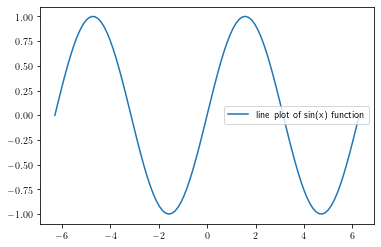
\includegraphics[scale=0.6]{legend.png}
\end{figure}

By default, the legend will appear in the top-right corner of the plot.
You can customize the location of the legend by using the \texttt{loc}
argument of the \texttt{plt.legend()} function. The \texttt{loc}
argument can be set to a string or integer value as given in the
following table:
$$
\begin{array}{|l|l|}
\hline
String & Integer \\
\hline
`best' & 0 \\
`upper right' & 1 \\
`upper left' & 2 \\
`lower left' & 3 \\
`lower right' & 4 \\
`right' & 5 \\
`center left' & 6 \\
`center right' & 7 \\
`lower center' & 8 \\
`upper center' & 9 \\
`center' & 10 \\
\hline
\end{array}$$

\hypertarget{the-plot-title-axis-labels}{%
\paragraph{The Plot Title Axis
Labels}\label{the-plot-title-axis-labels}}

To give a plot a title above its axes in Matplotlib, you can use the
\texttt{plt.title} function by passing a string containing the title.
Similarly, to label the \textbf{x-} and \textbf{y-axes}, you can use the
\texttt{plt.xlabel} and \texttt{plt.ylabel} functions by passing the
label text as string arguments.

You can also customize the font size of the title and labels using the
\texttt{fontsize} parameter. For example,

\begin{Shaded}
\begin{Highlighting}[]
\ImportTok{import}\NormalTok{ matplotlib.pyplot }\ImportTok{as}\NormalTok{ plt}
\ImportTok{import}\NormalTok{ numpy }\ImportTok{as}\NormalTok{ np}
\CommentTok{\# Create an array of x values from 0 to 2*pi with a step size of 0.1}
\NormalTok{x }\OperatorTok{=}\NormalTok{ np.linspace(}\OperatorTok{{-}}\DecValTok{2}\OperatorTok{*}\NormalTok{np.pi, }\DecValTok{2}\OperatorTok{*}\NormalTok{np.pi, }\DecValTok{100}\NormalTok{)}

\CommentTok{\# Calculate y values for the sin function}
\NormalTok{y }\OperatorTok{=}\NormalTok{ np.sin(x)}

\CommentTok{\# Plot the sine function}
\NormalTok{plt.plot(x, y,label}\OperatorTok{=}\StringTok{"line plot of sin(x) function"}\NormalTok{)}

\CommentTok{\# Calculate y values for the sin function}
\NormalTok{y }\OperatorTok{=}\NormalTok{ np.cos(x)}

\CommentTok{\# Plot the cosine function}
\NormalTok{plt.plot(x, y,label}\OperatorTok{=}\StringTok{"line plot of cosin(x) function"}\NormalTok{)}

\CommentTok{\# Add the legend to the plot}
\NormalTok{plt.legend()}
\CommentTok{\#Add a title}
\NormalTok{plt.title(}\StringTok{"sin(x) vs cosin(x) plots"}\NormalTok{)}
\CommentTok{\# Add lable to x axis and y axis}
\NormalTok{plt.xlabel(}\StringTok{"x values"}\NormalTok{, fontsize}\OperatorTok{=}\DecValTok{16}\NormalTok{)}
\NormalTok{plt.ylabel(}\StringTok{"y values"}\NormalTok{, fontsize}\OperatorTok{=}\DecValTok{16}\NormalTok{)}

\CommentTok{\# Diplay the result}
\NormalTok{plt.show()}
\end{Highlighting}
\end{Shaded}

\begin{figure}
\centering
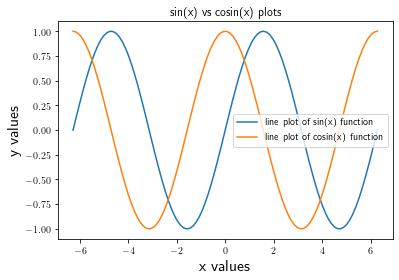
\includegraphics[scale=0.6]{xylabels.png}
\end{figure}

\hypertarget{using-latex-in-pyplot}{%
\paragraph{Using LATEX in pyplot}\label{using-latex-in-pyplot}}

You can use LaTeX syntax in your Matplotlib plot labels by enclosing the
LaTeX code within dollar signs (\texttt{\$\ \$}) in the label string.

However, you need to enable this option in Matplotlib's ``\emph{rc
settings}'' by calling
\texttt{plt.rc(\textquotesingle{}text\textquotesingle{},\ usetex=True)}.

Make sure you have LaTeX installed on your system to use LaTeX in your
plot labels.

To prevent Python from escaping any characters, use raw strings
\texttt{(r\textquotesingle{}xxx\textquotesingle{})}. For example,

\begin{Shaded}
\begin{Highlighting}[]
\ImportTok{import}\NormalTok{ matplotlib.pyplot }\ImportTok{as}\NormalTok{ plt}
\ImportTok{import}\NormalTok{ numpy }\ImportTok{as}\NormalTok{ np}
\CommentTok{\# Create an array of x values from 0 to 2*pi with a step size of 0.1}
\NormalTok{x }\OperatorTok{=}\NormalTok{ np.linspace(}\OperatorTok{{-}}\DecValTok{2}\OperatorTok{*}\NormalTok{np.pi, }\DecValTok{2}\OperatorTok{*}\NormalTok{np.pi, }\DecValTok{100}\NormalTok{)}

\CommentTok{\# Calculate y values for the sin function}
\NormalTok{y }\OperatorTok{=}\NormalTok{ np.sin(x)}

\CommentTok{\# Plot the sine function}
\NormalTok{plt.plot(x, y,label}\OperatorTok{=}\StringTok{"sin(x)"}\NormalTok{)}
\CommentTok{\#Activate LaTeX}
\NormalTok{plt.rc(}\StringTok{\textquotesingle{}text\textquotesingle{}}\NormalTok{, usetex}\OperatorTok{=}\VariableTok{True}\NormalTok{)}
\CommentTok{\# Add the legend to the plot}
\NormalTok{plt.legend()}
\CommentTok{\#Add a title}
\NormalTok{plt.title(}\VerbatimStringTok{r"$\textbackslash{}sin(x)=\textbackslash{}displaystyle\textbackslash{}sum\_\{i=0\}\^{}\{\textbackslash{}infty\}\{({-}1)\}\^{}n\textbackslash{}frac\{z\^{}\{2n+1}\SpecialCharTok{\}\}\{\{}\VerbatimStringTok{(2n+1)\}!\}$"}\NormalTok{,fontsize}\OperatorTok{=}\DecValTok{16}\NormalTok{)}
\CommentTok{\# Add lable to x axis and y axis}
\NormalTok{plt.xlabel(}\VerbatimStringTok{r"x values using \textbackslash{}LaTeX"}\NormalTok{, fontsize}\OperatorTok{=}\DecValTok{16}\NormalTok{)}
\NormalTok{plt.ylabel(}\VerbatimStringTok{r"y values "}\NormalTok{, fontsize}\OperatorTok{=}\DecValTok{12}\NormalTok{)}

\CommentTok{\# Diplay the result}
\NormalTok{plt.show()}
\end{Highlighting}
\end{Shaded}

\begin{figure}
\centering
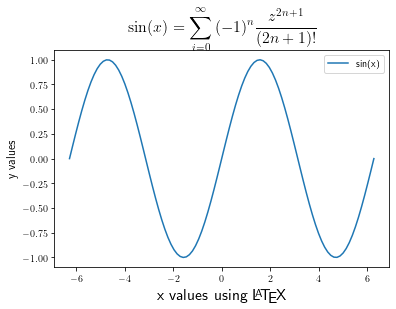
\includegraphics[scale=0.6]{Latex.png}
\end{figure}

\hypertarget{customizing-plots}{%
\subsection{Customizing Plots}\label{customizing-plots}}

\hypertarget{customize-figure}{%
\paragraph{Customize figure}\label{customize-figure}}

\texttt{plt.figure()} can take several arguments to customize the
created figure. Here are some of the common arguments:

$$\begin{array}{|l|l|}
\hline
  Argument&Description\\
\hline
\texttt{num} &\text{An identifier for the figure - if none is provided,}\\
&\text{ an integer, starting at 1, is used and incremented with each}\\
&\text{ figure created; alternatively, using a string will set the window}\\
&\text{ title to that string when the figure is displayed with plt.show() }\\
\texttt{figsize} &\text{A tuple of figure (width, height), in inches }\\
\texttt{dpi} &\text{Figure resolution in dots per inch }\\
\texttt{facecolor} &\text{Figure background color }\\
\texttt{edgecolor} &\text{Figure border color }\\
\hline
\end{array}$$

For example:

\begin{Shaded}
\begin{Highlighting}[]
\ImportTok{import}\NormalTok{ matplotlib.pyplot }\ImportTok{as}\NormalTok{ plt}
\ImportTok{import}\NormalTok{ numpy }\ImportTok{as}\NormalTok{ np}
\NormalTok{fig}\OperatorTok{=}\NormalTok{plt.figure(figsize}\OperatorTok{=}\NormalTok{(}\DecValTok{8}\NormalTok{,}\DecValTok{8}\NormalTok{),linewidth}\OperatorTok{=}\DecValTok{3}\NormalTok{,dpi}\OperatorTok{=}\DecValTok{150}\NormalTok{,edgecolor}\OperatorTok{=}\StringTok{"red"}\NormalTok{,facecolor}\OperatorTok{=}\StringTok{\textquotesingle{}cyan\textquotesingle{}}\NormalTok{)}
\NormalTok{x }\OperatorTok{=}\NormalTok{ np.linspace(}\OperatorTok{{-}}\DecValTok{2}\OperatorTok{*}\NormalTok{np.pi, }\DecValTok{2}\OperatorTok{*}\NormalTok{np.pi, }\DecValTok{100}\NormalTok{)}
\NormalTok{plt.plot(x,np.sin(x))}
\NormalTok{plt.plot(x,np.cos(x))}
\NormalTok{plt.show()}
\end{Highlighting}
\end{Shaded}

\begin{figure}
\centering
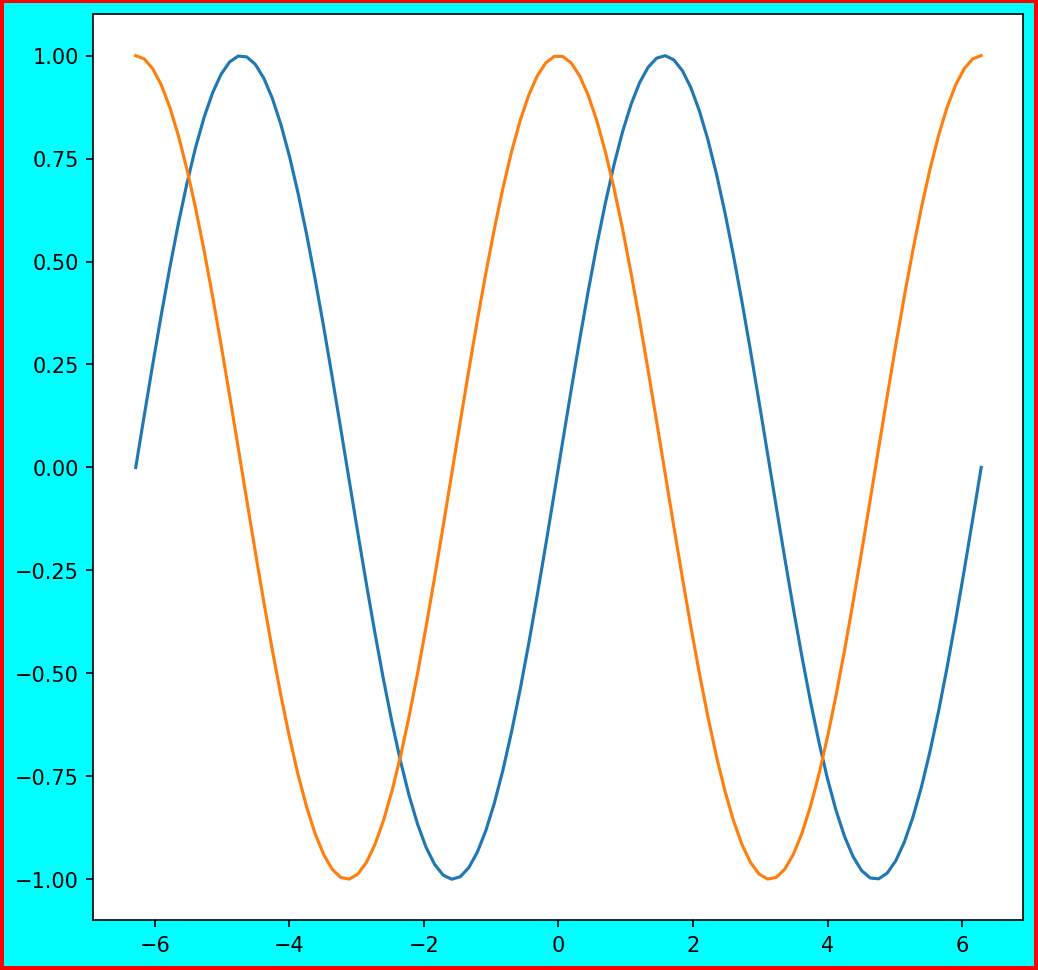
\includegraphics[scale=0.6]{fig_costum.png}
\end{figure}

\hypertarget{markers}{%
\paragraph{Markers}\label{markers}}

To customize markers in a plot using matplotlib library in Python, you
can use the marker parameter of the \texttt{plot()} function. By
default, the \texttt{plot()} function creates a line plot without any
markers on the data points.

To add a marker on each point of the plotted data, you can set the
marker parameter to the desired symbol. Here's an example code that
plots a simple line graph with circle markers:

\begin{Shaded}
\begin{Highlighting}[]
\ImportTok{import}\NormalTok{ matplotlib.pyplot }\ImportTok{as}\NormalTok{ plt}
\ImportTok{import}\NormalTok{ numpy }\ImportTok{as}\NormalTok{ np}

\CommentTok{\# Generate some sample data}
\NormalTok{x }\OperatorTok{=}\NormalTok{ np.arange(}\DecValTok{0}\NormalTok{, }\DecValTok{10}\NormalTok{, }\FloatTok{0.1}\NormalTok{)}
\NormalTok{y }\OperatorTok{=}\NormalTok{ np.sin(x)}

\CommentTok{\# Create a plot with circle markers}
\NormalTok{plt.plot(x, y, marker}\OperatorTok{=}\StringTok{\textquotesingle{}o\textquotesingle{}}\NormalTok{)}

\CommentTok{\# Show the plot}
\NormalTok{plt.show()}
\end{Highlighting}
\end{Shaded}

\begin{figure}
\centering
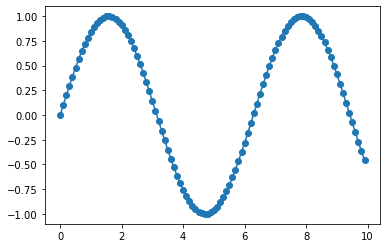
\includegraphics[scale=0.6]{marker_o.png}
\end{figure}

Other commonly used markers in the following table

$$\begin{array}{|l|l|l|}
\hline
Code & Marker & Description \\
\hline
. & \cdot & Point \\
o & \circ & Circle \\
+ & + & Plus \\
x & \times & Cross \\
D & \diamond & Diamond \\
v & \triangledown & \text{Downward triangle} \\
s & \Box & Square \\
* & \star & Star \\
\hline
\end{array}$$

Here are some of the most commonly used marker properties:

\begin{itemize}
\tightlist
\item
  \textbf{markersize (abbreviated ms)}: Specifies the size of the
  marker, in points.
\item
  \textbf{markevery}: Specifies how often a marker is shown on the plot.
  Set to a positive integer N to print a marker every N points; the
  default, None, prints a marker for every point.
\item
  \textbf{markerfacecolor (abbreviated mfc)}: Specifies the fill color
  of the marker.
\item
  \textbf{markeredgecolor (abbreviated mec)}: Specifies the edge color
  of the marker.
\item
  \textbf{markeredgewidth (abbreviated mew)}: Specifies the width of the
  marker edge, in points. For example:
\end{itemize}

\begin{Shaded}
\begin{Highlighting}[]
\ImportTok{import}\NormalTok{ numpy }\ImportTok{as}\NormalTok{ np}
\ImportTok{import}\NormalTok{ matplotlib.pyplot }\ImportTok{as}\NormalTok{ plt}

\CommentTok{\# Generate some sample data}
\NormalTok{x }\OperatorTok{=}\NormalTok{ np.linspace(}\DecValTok{0}\NormalTok{, }\DecValTok{10}\NormalTok{, }\DecValTok{100}\NormalTok{)}
\NormalTok{y }\OperatorTok{=}\NormalTok{ np.sin(x)}

\CommentTok{\# Plot the data with markers}
\NormalTok{plt.plot(x, y, marker}\OperatorTok{=}\StringTok{\textquotesingle{}o\textquotesingle{}}\NormalTok{, markersize}\OperatorTok{=}\DecValTok{8}\NormalTok{, markerfacecolor}\OperatorTok{=}\StringTok{\textquotesingle{}red\textquotesingle{}}\NormalTok{, markeredgecolor}\OperatorTok{=}\StringTok{\textquotesingle{}black\textquotesingle{}}\NormalTok{, markeredgewidth}\OperatorTok{=}\DecValTok{1}\NormalTok{)}

\CommentTok{\# Add some labels and a title}
\NormalTok{plt.xlabel(}\StringTok{\textquotesingle{}X\textquotesingle{}}\NormalTok{)}
\NormalTok{plt.ylabel(}\StringTok{\textquotesingle{}Y\textquotesingle{}}\NormalTok{)}
\NormalTok{plt.title(}\StringTok{\textquotesingle{}Sample Plot\textquotesingle{}}\NormalTok{)}

\CommentTok{\# Show the plot}
\NormalTok{plt.show()}
\end{Highlighting}
\end{Shaded}

\begin{figure}
\centering
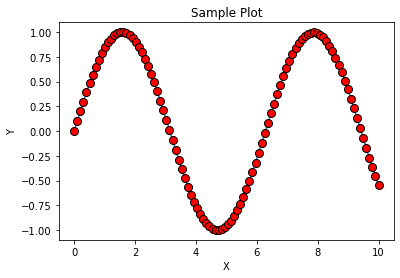
\includegraphics[scale=0.6]{marker_prop.png}
\end{figure}

\hypertarget{colors}{%
\paragraph{Colors}\label{colors}}

In Matplotlib, you can customize the color of plotted lines using the
\texttt{color} parameter. There are several ways to specify a color:

\begin{enumerate}
\def\labelenumi{\arabic{enumi}.}
\item
  One-letter codes: You can use one-letter codes to represent some
  common colors, as shown in the table above. For example, color=`r'
  specifies a red line and markers.
\item
  Tableau color sequence: Since Matplotlib 2.0, the default color
  sequence for a series of lines on the same plot is the more pleasing
  ``Tableau'' sequence. The string identifiers for Tableau colors are
  also given in the table above.
\item
  Shades of gray: You can specify shades of gray using a string
  representing a float in the range 0--1. Here, 0 represents black and 1
  represents white.
\item
  HTML hex strings: You can use HTML hex strings to represent colors
  using their red, green, and blue (RGB) components in the range
  00--ff.~For example, color=`\#ff00ff' is magenta.
\item
  RGB tuples: You can also pass RGB components as a tuple of three
  values in the range 0--1. For example, color=(0.5, 0., 0.) represents
  a dark red color.
\end{enumerate}

$$\begin{array}{|l|l|}
\hline
  \text{Basic color codes} & \text{Tableau colors}\\
\hline
b = blue & tab:blue \\
g = green & tab:orange \\
r = red & tab:green \\
c = cyan & tab:red \\
m = magenta & tab:purple \\
y = yellow & tab:brown \\
k = black & tab:pink \\
w = white & tab:gray \\
& tab:olive \\
& tab:cyan \\
\hline
\end{array}
$$

Here's an example code that shows how to use different color formats:

\begin{Shaded}
\begin{Highlighting}[]
\ImportTok{import}\NormalTok{ matplotlib.pyplot }\ImportTok{as}\NormalTok{ plt}
\ImportTok{import}\NormalTok{ numpy }\ImportTok{as}\NormalTok{ np}

\CommentTok{\# Generate some sample data}
\NormalTok{x }\OperatorTok{=}\NormalTok{ np.arange(}\DecValTok{0}\NormalTok{, }\DecValTok{10}\NormalTok{, }\FloatTok{0.1}\NormalTok{)}
\NormalTok{y }\OperatorTok{=}\NormalTok{ np.sin(x)}

\CommentTok{\# Create a plot with different colors}
\NormalTok{fig, ax }\OperatorTok{=}\NormalTok{ plt.subplots()}
\NormalTok{ax.plot(x, x}\OperatorTok{**}\DecValTok{2}\OperatorTok{*}\NormalTok{y, color}\OperatorTok{=}\StringTok{\textquotesingle{}b\textquotesingle{}}\NormalTok{, label}\OperatorTok{=}\StringTok{\textquotesingle{}Blue line\textquotesingle{}}\NormalTok{)}
\NormalTok{ax.plot(x, }\OperatorTok{{-}}\NormalTok{x}\OperatorTok{**}\DecValTok{2}\OperatorTok{*}\NormalTok{y, color}\OperatorTok{=}\StringTok{\textquotesingle{}\#ff00ff\textquotesingle{}}\NormalTok{, label}\OperatorTok{=}\StringTok{\textquotesingle{}Magenta line\textquotesingle{}}\NormalTok{)}
\NormalTok{ax.plot(x, }\FloatTok{0.5}\OperatorTok{*}\NormalTok{x}\OperatorTok{**}\DecValTok{2} \OperatorTok{*}\NormalTok{ y, color}\OperatorTok{=}\NormalTok{(}\FloatTok{0.5}\NormalTok{, }\FloatTok{0.}\NormalTok{, }\FloatTok{0.}\NormalTok{), label}\OperatorTok{=}\StringTok{\textquotesingle{}Dark red line\textquotesingle{}}\NormalTok{)}
\NormalTok{ax.plot(x, }\OperatorTok{{-}}\FloatTok{0.5} \OperatorTok{*}\NormalTok{x}\OperatorTok{**}\DecValTok{2} \OperatorTok{*}\NormalTok{ y, color}\OperatorTok{=}\StringTok{\textquotesingle{}tab:green\textquotesingle{}}\NormalTok{, label}\OperatorTok{=}\StringTok{\textquotesingle{}Tableau green line\textquotesingle{}}\NormalTok{)}

\CommentTok{\# Set axis labels and legend}
\NormalTok{ax.set\_xlabel(}\StringTok{\textquotesingle{}X\textquotesingle{}}\NormalTok{)}
\NormalTok{ax.set\_ylabel(}\StringTok{\textquotesingle{}Y\textquotesingle{}}\NormalTok{)}
\NormalTok{ax.legend()}

\CommentTok{\# Show the plot}
\NormalTok{plt.show()}
\end{Highlighting}
\end{Shaded}

\begin{figure}
\centering
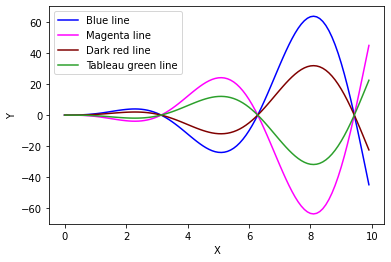
\includegraphics[scale=0.6]{line_color.png}
\end{figure}

\hypertarget{line-styles-and-widths}{%
\paragraph{Line Styles and Widths}\label{line-styles-and-widths}}

Matplotlib provides several different line styles for plotting data. The
line style can be specified using the linestyle argument of the
\texttt{plot()} function. The default line style is a solid line, but
there are several other styles available, such as dashed, dotted, and
dash-dot.

In addition to line styles, you can also specify the width of the line
using the linewidth argument.

Here's an example of how to use line styles and widths in Matplotlib:

\begin{Shaded}
\begin{Highlighting}[]
\ImportTok{import}\NormalTok{ numpy }\ImportTok{as}\NormalTok{ np}
\ImportTok{import}\NormalTok{ matplotlib.pyplot }\ImportTok{as}\NormalTok{ plt}

\CommentTok{\# Generate some sample data}
\NormalTok{x }\OperatorTok{=}\NormalTok{ np.linspace(}\DecValTok{0}\NormalTok{, }\DecValTok{10}\NormalTok{, }\DecValTok{100}\NormalTok{)}
\NormalTok{y }\OperatorTok{=}\NormalTok{ np.sin(x)}

\CommentTok{\# Plot the data with different line styles and widths}
\NormalTok{plt.plot(x, y, linestyle}\OperatorTok{=}\StringTok{\textquotesingle{}{-}\textquotesingle{}}\NormalTok{, linewidth}\OperatorTok{=}\DecValTok{1}\NormalTok{, label}\OperatorTok{=}\StringTok{\textquotesingle{}Solid\textquotesingle{}}\NormalTok{)}
\NormalTok{plt.plot(x }\OperatorTok{+} \FloatTok{0.5}\NormalTok{, y, linestyle}\OperatorTok{=}\StringTok{\textquotesingle{}{-}{-}\textquotesingle{}}\NormalTok{, linewidth}\OperatorTok{=}\DecValTok{2}\NormalTok{, label}\OperatorTok{=}\StringTok{\textquotesingle{}Dashed\textquotesingle{}}\NormalTok{)}
\NormalTok{plt.plot(x }\OperatorTok{+} \DecValTok{1}\NormalTok{, y, linestyle}\OperatorTok{=}\StringTok{\textquotesingle{}{-}.\textquotesingle{}}\NormalTok{, linewidth}\OperatorTok{=}\DecValTok{3}\NormalTok{, label}\OperatorTok{=}\StringTok{\textquotesingle{}Dash{-}Dot\textquotesingle{}}\NormalTok{)}
\NormalTok{plt.plot(x }\OperatorTok{+} \FloatTok{1.5}\NormalTok{, y, linestyle}\OperatorTok{=}\StringTok{\textquotesingle{}:\textquotesingle{}}\NormalTok{, linewidth}\OperatorTok{=}\DecValTok{4}\NormalTok{, label}\OperatorTok{=}\StringTok{\textquotesingle{}Dotted\textquotesingle{}}\NormalTok{)}

\CommentTok{\# Add a legend and a title}
\NormalTok{plt.legend()}
\NormalTok{plt.title(}\StringTok{\textquotesingle{}Line Styles and Widths\textquotesingle{}}\NormalTok{)}

\CommentTok{\# Show the plot}
\NormalTok{plt.show()}
\end{Highlighting}
\end{Shaded}

This will produce a plot with four different line styles and widths, as
shown below: 
\begin{figure}
  \centering
  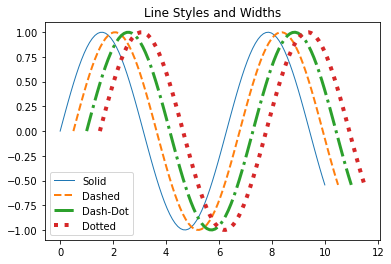
\includegraphics[scale=0.6]{line_custom.png}
\end{figure}

Here is a table of some of the most commonly used line styles in
Matplotlib:

$$\begin{array}{|l|l|}
\hline
  Code & \text{Line style description}\\
\hline
'-' & \text{Solid line }\\
'--' & \text{Dashed line }\\
'-.' & \text{Dash-dot line }\\
':' & \text{Dotted line }\\
\hline
\end{array}
$$

\hypertarget{plot-limits}{%
\paragraph{Plot Limits}\label{plot-limits}}

When you plot data in Matplotlib, the plot will automatically adjust the
axis limits to fit the data. However, sometimes you may want to set the
axis limits yourself to focus on a particular range of the data.

You can set the limits of the x-axis and y-axis using the
\texttt{xlim()} and \texttt{ylim()} functions, respectively. Both
functions take two arguments, the lower and upper bounds of the axis
limits.

Here's an example of how to set plot limits in Matplotlib:

\begin{Shaded}
\begin{Highlighting}[]
\ImportTok{import}\NormalTok{ numpy }\ImportTok{as}\NormalTok{ np}
\ImportTok{import}\NormalTok{ matplotlib.pyplot }\ImportTok{as}\NormalTok{ plt}

\CommentTok{\# Generate some sample data}
\NormalTok{x }\OperatorTok{=}\NormalTok{ np.linspace(}\DecValTok{0}\NormalTok{, }\DecValTok{10}\NormalTok{, }\DecValTok{100}\NormalTok{)}
\NormalTok{y }\OperatorTok{=}\NormalTok{ np.sin(x)}

\CommentTok{\# Plot the data}
\NormalTok{plt.plot(x, y)}

\CommentTok{\# Set the x{-}axis limits to [2, 8]}
\NormalTok{plt.xlim(}\DecValTok{2}\NormalTok{, }\DecValTok{8}\NormalTok{)}

\CommentTok{\# Set the y{-}axis limits to [{-}1, 1]}
\NormalTok{plt.ylim(}\OperatorTok{{-}}\DecValTok{1}\NormalTok{, }\DecValTok{1}\NormalTok{)}

\CommentTok{\# Add a title and axis labels}
\NormalTok{plt.title(}\StringTok{\textquotesingle{}Plot Limits Example\textquotesingle{}}\NormalTok{)}
\NormalTok{plt.xlabel(}\StringTok{\textquotesingle{}x\textquotesingle{}}\NormalTok{)}
\NormalTok{plt.ylabel(}\StringTok{\textquotesingle{}y\textquotesingle{}}\NormalTok{)}

\CommentTok{\# Show the plot}
\NormalTok{plt.show()}
\end{Highlighting}
\end{Shaded}

This will produce a plot with x-axis limits of {[}2, 8{]} and y-axis
limits of {[}-1, 1{]}, as shown below: 
\begin{figure}
  \centering
  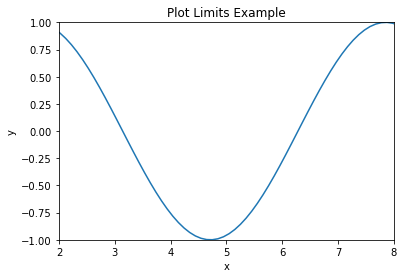
\includegraphics[scale=0.6]{plot_lim.png}
\end{figure}

\hypertarget{tick-marks}{%
\paragraph{Tick marks}\label{tick-marks}}

When you plot data in Matplotlib, the plot will automatically generate
tick marks on the x-axis and y-axis to help label the plot. These tick
marks are the small lines or marks on the axes that indicate the value
at a particular location.

You can customize the tick marks using various functions in Matplotlib.
The \texttt{xticks()} and \texttt{yticks()} functions allow you to set
the locations and labels of the tick marks on the x-axis and y-axis,
respectively.

Here's an example of how to customize tick marks in Matplotlib:

\begin{Shaded}
\begin{Highlighting}[]
\ImportTok{import}\NormalTok{ numpy }\ImportTok{as}\NormalTok{ np}
\ImportTok{import}\NormalTok{ matplotlib.pyplot }\ImportTok{as}\NormalTok{ plt}

\CommentTok{\# Generate some sample data}
\NormalTok{x }\OperatorTok{=}\NormalTok{ np.linspace(}\DecValTok{0}\NormalTok{, }\DecValTok{10}\OperatorTok{*}\NormalTok{np.pi, }\DecValTok{100}\NormalTok{)}
\NormalTok{y }\OperatorTok{=}\NormalTok{ np.sin(x)}

\CommentTok{\# Plot the data}
\NormalTok{plt.plot(x, y)}

\CommentTok{\# Set the x{-}axis tick marks to be [0, 2*pi, 4*pi, 6*pi, 8*pi, 10*pi]}
\NormalTok{plt.xticks([}\DecValTok{0}\NormalTok{, }\DecValTok{2}\OperatorTok{*}\NormalTok{np.pi, }\DecValTok{4}\OperatorTok{*}\NormalTok{np.pi, }\DecValTok{6}\OperatorTok{*}\NormalTok{np.pi, }\DecValTok{8}\OperatorTok{*}\NormalTok{np.pi, }\DecValTok{10}\OperatorTok{*}\NormalTok{np.pi], [}\StringTok{\textquotesingle{}0\textquotesingle{}}\NormalTok{, }\VerbatimStringTok{r\textquotesingle{}$2\textbackslash{}pi$\textquotesingle{}}\NormalTok{, }\VerbatimStringTok{r\textquotesingle{}$4\textbackslash{}pi$\textquotesingle{}}\NormalTok{, }\VerbatimStringTok{r\textquotesingle{}$6\textbackslash{}pi$\textquotesingle{}}\NormalTok{, }\VerbatimStringTok{r\textquotesingle{}$8\textbackslash{}pi$\textquotesingle{}}\NormalTok{, }\VerbatimStringTok{r\textquotesingle{}$10\textbackslash{}pi$\textquotesingle{}}\NormalTok{])}

\CommentTok{\# Set the y{-}axis tick marks to be [{-}1, 0, 1]}
\NormalTok{plt.yticks([}\OperatorTok{{-}}\DecValTok{1}\NormalTok{, }\DecValTok{0}\NormalTok{, }\DecValTok{1}\NormalTok{], [}\StringTok{\textquotesingle{}{-}1\textquotesingle{}}\NormalTok{, }\StringTok{\textquotesingle{}0\textquotesingle{}}\NormalTok{, }\StringTok{\textquotesingle{}1\textquotesingle{}}\NormalTok{])}

\CommentTok{\# Add a title and axis labels}
\NormalTok{plt.title(}\StringTok{\textquotesingle{}Ticks Example\textquotesingle{}}\NormalTok{)}
\NormalTok{plt.xlabel(}\StringTok{\textquotesingle{}x\textquotesingle{}}\NormalTok{)}
\NormalTok{plt.ylabel(}\StringTok{\textquotesingle{}y\textquotesingle{}}\NormalTok{)}

\CommentTok{\# Show the plot}
\NormalTok{plt.show()}
\end{Highlighting}
\end{Shaded}

This will produce a plot with custom tick marks on both the x-axis and
y-axis, as shown below: 
\begin{figure}
  \centering
  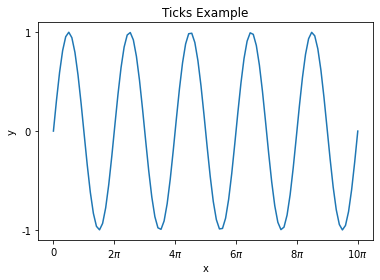
\includegraphics[scale=0.6]{ticks.png}
\end{figure}

\hypertarget{more-advanced-plotting}{%
\section{More Advanced Plotting}\label{more-advanced-plotting}}

\hypertarget{polar-plots}{%
\subsection{Polar Plots}\label{polar-plots}}

Polar plots are a type of plot where data is plotted on a polar
coordinate system instead of a Cartesian coordinate system. Polar plots
are useful for visualizing data that is cyclical in nature. To create a
polar plot, you can use the \texttt{plt.polar()} function. For example:

\begin{Shaded}
\begin{Highlighting}[]
\ImportTok{import}\NormalTok{ matplotlib.pyplot }\ImportTok{as}\NormalTok{ plt}
\ImportTok{import}\NormalTok{ numpy }\ImportTok{as}\NormalTok{ np}

\NormalTok{theta }\OperatorTok{=}\NormalTok{ np.linspace(}\DecValTok{0}\NormalTok{, }\DecValTok{2}\OperatorTok{*}\NormalTok{np.pi, }\DecValTok{100}\NormalTok{)}
\NormalTok{r }\OperatorTok{=}\NormalTok{ np.sin(}\DecValTok{5}\OperatorTok{*}\NormalTok{theta)}

\NormalTok{plt.polar(theta, r)}
\NormalTok{plt.show()}
\end{Highlighting}
\end{Shaded}

This will create a polar plot of a sine wave with five complete cycles:
\begin{figure}
  \centering
  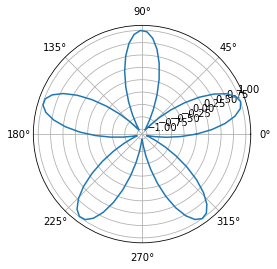
\includegraphics[scale=0.6]{polar.png}
\end{figure}

\hypertarget{histograms}{%
\subsection{Histograms}\label{histograms}}

Histograms are a way to visualize the distribution of a set of data.
They work by dividing the data into a set of intervals, or ``bins,'' and
then counting the number of data points that fall into each bin. To
create a histogram in Matplotlib, you can use the \texttt{plt.hist()}
function. For example:

\begin{Shaded}
\begin{Highlighting}[]
\ImportTok{import}\NormalTok{ matplotlib.pyplot }\ImportTok{as}\NormalTok{ plt}
\ImportTok{import}\NormalTok{ numpy }\ImportTok{as}\NormalTok{ np}

\NormalTok{data }\OperatorTok{=}\NormalTok{ np.random.normal(}\DecValTok{0}\NormalTok{, }\DecValTok{1}\NormalTok{, }\DecValTok{1000}\NormalTok{)}

\NormalTok{plt.hist(data, bins}\OperatorTok{=}\DecValTok{30}\NormalTok{)}
\NormalTok{plt.show()}
\end{Highlighting}
\end{Shaded}

\begin{figure}
  \centering
  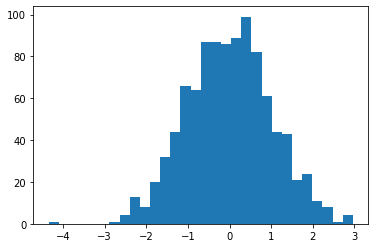
\includegraphics[scale=0.6]{hist.png} 
\end{figure}

\hypertarget{BarPlot}{%
\subsection{Bar Plot}\label{BarPlot}}

Bar plots are used to compare
different categories of data. They work by plotting bars of different
heights to represent the values associated with each category. To create
a bar plot in Matplotlib, you can use the plt.bar() function. For
example:

\begin{Shaded}
\begin{Highlighting}[]
\ImportTok{import}\NormalTok{ matplotlib.pyplot }\ImportTok{as}\NormalTok{ plt}
\ImportTok{import}\NormalTok{ numpy }\ImportTok{as}\NormalTok{ np}

\NormalTok{data }\OperatorTok{=}\NormalTok{ [}\DecValTok{25}\NormalTok{, }\DecValTok{50}\NormalTok{, }\DecValTok{75}\NormalTok{, }\DecValTok{100}\NormalTok{]}

\NormalTok{plt.bar(}\BuiltInTok{range}\NormalTok{(}\BuiltInTok{len}\NormalTok{(data)), data)}
\NormalTok{plt.xticks(}\BuiltInTok{range}\NormalTok{(}\BuiltInTok{len}\NormalTok{(data)), [}\StringTok{\textquotesingle{}A\textquotesingle{}}\NormalTok{, }\StringTok{\textquotesingle{}B\textquotesingle{}}\NormalTok{, }\StringTok{\textquotesingle{}C\textquotesingle{}}\NormalTok{, }\StringTok{\textquotesingle{}D\textquotesingle{}}\NormalTok{])}
\NormalTok{plt.show()}
\end{Highlighting}
\end{Shaded}

\begin{figure}
\centering
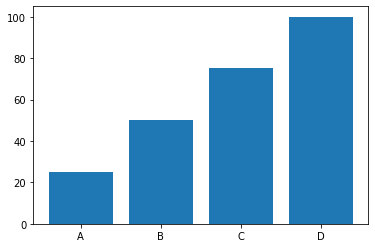
\includegraphics[scale=0.6]{bar.png}
\end{figure}

    \begin{tcolorbox}[breakable, size=fbox, boxrule=1pt, pad at break*=1mm,colback=cellbackground, colframe=cellborder]
\prompt{In}{incolor}{12}{\boxspacing}
\begin{Verbatim}[commandchars=\\\{\}]
\PY{c+c1}{\PYZsh{}https://home.agh.edu.pl/\PYZti{}mariuszp/wfiis\PYZus{}stw/Learning\PYZus{}Scientific\PYZus{}Programming\PYZus{}with\PYZus{}Python\PYZus{}2ed\PYZus{}Ch\PYZus{}Hill\PYZus{}Cambridge\PYZus{}2020.pdf}
\PY{k+kn}{import} \PY{n+nn}{numpy} \PY{k}{as} \PY{n+nn}{np}
\PY{k+kn}{from} \PY{n+nn}{matplotlib} \PY{k+kn}{import} \PY{n}{pyplot} \PY{k}{as} \PY{n}{plt}
\PY{n}{mean} \PY{o}{=} \PY{l+m+mi}{0}\PY{p}{;} \PY{n}{std} \PY{o}{=} \PY{n}{np}\PY{o}{.}\PY{n}{array}\PY{p}{(}\PY{p}{[}\PY{l+m+mi}{1}\PY{p}{,}\PY{l+m+mf}{1.5}\PY{p}{,}\PY{l+m+mi}{2}\PY{p}{]}\PY{p}{)}\PY{p}{;} \PY{n}{variance} \PY{o}{=} \PY{n}{np}\PY{o}{.}\PY{n}{square}\PY{p}{(}\PY{n}{std}\PY{p}{[}\PY{l+m+mi}{0}\PY{p}{]}\PY{p}{)}
\PY{n}{x} \PY{o}{=} \PY{n}{np}\PY{o}{.}\PY{n}{arange}\PY{p}{(}\PY{o}{\PYZhy{}}\PY{l+m+mi}{5}\PY{p}{,}\PY{l+m+mi}{5}\PY{p}{,}\PY{l+m+mf}{.01}\PY{p}{)}
\PY{n}{f1} \PY{o}{=} \PY{n}{np}\PY{o}{.}\PY{n}{exp}\PY{p}{(}\PY{o}{\PYZhy{}}\PY{n}{np}\PY{o}{.}\PY{n}{square}\PY{p}{(}\PY{n}{x}\PY{o}{\PYZhy{}}\PY{n}{mean}\PY{p}{)}\PY{o}{/}\PY{l+m+mi}{2}\PY{o}{*}\PY{n}{variance}\PY{p}{)}\PY{o}{/}\PY{p}{(}\PY{n}{np}\PY{o}{.}\PY{n}{sqrt}\PY{p}{(}\PY{l+m+mi}{2}\PY{o}{*}\PY{n}{np}\PY{o}{.}\PY{n}{pi}\PY{o}{*}\PY{n}{variance}\PY{p}{)}\PY{p}{)}
\PY{n}{variance} \PY{o}{=} \PY{n}{np}\PY{o}{.}\PY{n}{square}\PY{p}{(}\PY{n}{std}\PY{p}{[}\PY{l+m+mi}{1}\PY{p}{]}\PY{p}{)}
\PY{n}{f2}\PY{o}{=} \PY{n}{np}\PY{o}{.}\PY{n}{exp}\PY{p}{(}\PY{o}{\PYZhy{}}\PY{n}{np}\PY{o}{.}\PY{n}{square}\PY{p}{(}\PY{n}{x}\PY{o}{\PYZhy{}}\PY{n}{mean}\PY{p}{)}\PY{o}{/}\PY{l+m+mi}{2}\PY{o}{*}\PY{n}{variance}\PY{p}{)}\PY{o}{/}\PY{p}{(}\PY{n}{np}\PY{o}{.}\PY{n}{sqrt}\PY{p}{(}\PY{l+m+mi}{2}\PY{o}{*}\PY{n}{np}\PY{o}{.}\PY{n}{pi}\PY{o}{*}\PY{n}{variance}\PY{p}{)}\PY{p}{)}
\PY{n}{variance} \PY{o}{=} \PY{n}{np}\PY{o}{.}\PY{n}{square}\PY{p}{(}\PY{n}{std}\PY{p}{[}\PY{l+m+mi}{2}\PY{p}{]}\PY{p}{)}
\PY{n}{f3}\PY{o}{=} \PY{n}{np}\PY{o}{.}\PY{n}{exp}\PY{p}{(}\PY{o}{\PYZhy{}}\PY{n}{np}\PY{o}{.}\PY{n}{square}\PY{p}{(}\PY{n}{x}\PY{o}{\PYZhy{}}\PY{n}{mean}\PY{p}{)}\PY{o}{/}\PY{l+m+mi}{2}\PY{o}{*}\PY{n}{variance}\PY{p}{)}\PY{o}{/}\PY{p}{(}\PY{n}{np}\PY{o}{.}\PY{n}{sqrt}\PY{p}{(}\PY{l+m+mi}{2}\PY{o}{*}\PY{n}{np}\PY{o}{.}\PY{n}{pi}\PY{o}{*}\PY{n}{variance}\PY{p}{)}\PY{p}{)}
\PY{n}{plt}\PY{o}{.}\PY{n}{plot}\PY{p}{(}\PY{n}{x}\PY{p}{,}\PY{n}{f1}\PY{p}{)}
\PY{n}{plt}\PY{o}{.}\PY{n}{plot}\PY{p}{(}\PY{n}{x}\PY{p}{,}\PY{n}{f2}\PY{p}{)}
\PY{n}{plt}\PY{o}{.}\PY{n}{plot}\PY{p}{(}\PY{n}{x}\PY{p}{,}\PY{n}{f3}\PY{p}{)}
\PY{n}{plt}\PY{o}{.}\PY{n}{ylabel}\PY{p}{(}\PY{l+s+s1}{\PYZsq{}}\PY{l+s+s1}{gaussian distribution}\PY{l+s+s1}{\PYZsq{}}\PY{p}{)}
\PY{n}{plt}\PY{o}{.}\PY{n}{show}\PY{p}{(}\PY{p}{)}
\end{Verbatim}
\end{tcolorbox}

    \begin{center}
    \adjustimage{max size={0.5\linewidth}{0.9\paperheight}}{output_1_0.png}
    \end{center}
    { \hspace*{\fill} \\}
    
    \begin{tcolorbox}[breakable, size=fbox, boxrule=1pt, pad at break*=1mm,colback=cellbackground, colframe=cellborder]
\prompt{In}{incolor}{3}{\boxspacing}
\begin{Verbatim}[commandchars=\\\{\}]
\PY{k+kn}{import} \PY{n+nn}{matplotlib}\PY{n+nn}{.}\PY{n+nn}{pyplot} \PY{k}{as} \PY{n+nn}{plt}
\PY{k+kn}{import} \PY{n+nn}{numpy} \PY{k}{as} \PY{n+nn}{np}
\PY{n}{fig}\PY{o}{=}\PY{n}{plt}\PY{o}{.}\PY{n}{figure}\PY{p}{(}\PY{n}{figsize}\PY{o}{=}\PY{p}{(}\PY{l+m+mi}{8}\PY{p}{,}\PY{l+m+mi}{6}\PY{p}{)}\PY{p}{)}
\PY{n}{x}\PY{o}{=}\PY{n}{np}\PY{o}{.}\PY{n}{linspace}\PY{p}{(}\PY{o}{\PYZhy{}}\PY{l+m+mi}{10}\PY{p}{,}\PY{l+m+mi}{10}\PY{p}{,}\PY{l+m+mi}{100}\PY{p}{)}

\PY{n}{ax1} \PY{o}{=} \PY{n}{fig}\PY{o}{.}\PY{n}{add\PYZus{}subplot}\PY{p}{(}\PY{l+m+mi}{3}\PY{p}{,} \PY{l+m+mi}{2}\PY{p}{,} \PY{l+m+mi}{1}\PY{p}{)}
\PY{n}{ax2} \PY{o}{=} \PY{n}{fig}\PY{o}{.}\PY{n}{add\PYZus{}subplot}\PY{p}{(}\PY{l+m+mi}{3}\PY{p}{,} \PY{l+m+mi}{2}\PY{p}{,} \PY{l+m+mi}{2}\PY{p}{)}
\PY{n}{ax3} \PY{o}{=} \PY{n}{fig}\PY{o}{.}\PY{n}{add\PYZus{}subplot}\PY{p}{(}\PY{l+m+mi}{3}\PY{p}{,} \PY{l+m+mi}{2}\PY{p}{,} \PY{l+m+mi}{3}\PY{p}{)}
\PY{n}{ax4} \PY{o}{=} \PY{n}{fig}\PY{o}{.}\PY{n}{add\PYZus{}subplot}\PY{p}{(}\PY{l+m+mi}{3}\PY{p}{,} \PY{l+m+mi}{2}\PY{p}{,} \PY{l+m+mi}{5}\PY{p}{)}


\PY{n}{ax1}\PY{o}{.}\PY{n}{plot}\PY{p}{(}\PY{n}{x}\PY{p}{,}\PY{n}{np}\PY{o}{.}\PY{n}{power}\PY{p}{(}\PY{n}{x}\PY{p}{,}\PY{l+m+mf}{1.}\PY{p}{)}\PY{o}{*}\PY{n}{np}\PY{o}{.}\PY{n}{sin}\PY{p}{(}\PY{n}{x}\PY{p}{)}\PY{p}{)}
\PY{n}{ax2}\PY{o}{.}\PY{n}{scatter}\PY{p}{(}\PY{n}{x}\PY{p}{,}\PY{n}{np}\PY{o}{.}\PY{n}{power}\PY{p}{(}\PY{n}{x}\PY{p}{,}\PY{l+m+mf}{2.}\PY{p}{)}\PY{o}{*}\PY{n}{np}\PY{o}{.}\PY{n}{sin}\PY{p}{(}\PY{n}{x}\PY{p}{)}\PY{p}{)}
\PY{n}{ax3}\PY{o}{.}\PY{n}{plot}\PY{p}{(}\PY{n}{x}\PY{p}{,}\PY{n}{np}\PY{o}{.}\PY{n}{power}\PY{p}{(}\PY{n}{x}\PY{p}{,}\PY{l+m+mf}{3.}\PY{p}{)}\PY{o}{*}\PY{n}{np}\PY{o}{.}\PY{n}{sin}\PY{p}{(}\PY{n}{x}\PY{p}{)}\PY{p}{)}
\PY{n}{ax4}\PY{o}{.}\PY{n}{plot}\PY{p}{(}\PY{n}{x}\PY{p}{,}\PY{n}{np}\PY{o}{.}\PY{n}{power}\PY{p}{(}\PY{n}{x}\PY{p}{,}\PY{l+m+mf}{4.}\PY{p}{)}\PY{o}{*}\PY{n}{np}\PY{o}{.}\PY{n}{sin}\PY{p}{(}\PY{n}{x}\PY{p}{)}\PY{p}{)}
\PY{n}{plt}\PY{o}{.}\PY{n}{show}\PY{p}{(}\PY{p}{)}
\end{Verbatim}
\end{tcolorbox}

    \begin{center}
    \adjustimage{max size={0.5\linewidth}{0.9\paperheight}}{output_2_0.png}
    \end{center}
    { \hspace*{\fill} \\}
    
    \begin{tcolorbox}[breakable, size=fbox, boxrule=1pt, pad at break*=1mm,colback=cellbackground, colframe=cellborder]
\prompt{In}{incolor}{20}{\boxspacing}
\begin{Verbatim}[commandchars=\\\{\}]
\PY{k+kn}{import} \PY{n+nn}{numpy} \PY{k}{as} \PY{n+nn}{np}
\PY{k+kn}{import} \PY{n+nn}{matplotlib}\PY{n+nn}{.}\PY{n+nn}{pyplot} \PY{k}{as} \PY{n+nn}{plt}

\PY{c+c1}{\PYZsh{} Generate some sample data}
\PY{n}{x} \PY{o}{=} \PY{n}{np}\PY{o}{.}\PY{n}{linspace}\PY{p}{(}\PY{l+m+mi}{0}\PY{p}{,} \PY{l+m+mi}{10}\PY{o}{*}\PY{n}{np}\PY{o}{.}\PY{n}{pi}\PY{p}{,} \PY{l+m+mi}{100}\PY{p}{)}
\PY{n}{y} \PY{o}{=} \PY{n}{np}\PY{o}{.}\PY{n}{sin}\PY{p}{(}\PY{n}{x}\PY{p}{)}

\PY{c+c1}{\PYZsh{} Plot the data}
\PY{n}{plt}\PY{o}{.}\PY{n}{plot}\PY{p}{(}\PY{n}{x}\PY{p}{,} \PY{n}{y}\PY{p}{)}

\PY{c+c1}{\PYZsh{} Set the x\PYZhy{}axis tick marks to be [0, 2*pi, 4*pi, 6*pi, 8*pi, 10*pi]}
\PY{n}{plt}\PY{o}{.}\PY{n}{xticks}\PY{p}{(}\PY{p}{[}\PY{l+m+mi}{0}\PY{p}{,} \PY{l+m+mi}{2}\PY{o}{*}\PY{n}{np}\PY{o}{.}\PY{n}{pi}\PY{p}{,} \PY{l+m+mi}{4}\PY{o}{*}\PY{n}{np}\PY{o}{.}\PY{n}{pi}\PY{p}{,} \PY{l+m+mi}{6}\PY{o}{*}\PY{n}{np}\PY{o}{.}\PY{n}{pi}\PY{p}{,} \PY{l+m+mi}{8}\PY{o}{*}\PY{n}{np}\PY{o}{.}\PY{n}{pi}\PY{p}{,} \PY{l+m+mi}{10}\PY{o}{*}\PY{n}{np}\PY{o}{.}\PY{n}{pi}\PY{p}{]}\PY{p}{,} \PY{p}{[}\PY{l+s+s1}{\PYZsq{}}\PY{l+s+s1}{10}\PY{l+s+s1}{\PYZsq{}}\PY{p}{,} \PY{l+s+sa}{r}\PY{l+s+s1}{\PYZsq{}}\PY{l+s+s1}{\PYZdl{}2}\PY{l+s+s1}{\PYZbs{}}\PY{l+s+s1}{pi\PYZdl{}}\PY{l+s+s1}{\PYZsq{}}\PY{p}{,} \PY{l+s+sa}{r}\PY{l+s+s1}{\PYZsq{}}\PY{l+s+s1}{\PYZdl{}4}\PY{l+s+s1}{\PYZbs{}}\PY{l+s+s1}{pi\PYZdl{}}\PY{l+s+s1}{\PYZsq{}}\PY{p}{,} \PY{l+s+sa}{r}\PY{l+s+s1}{\PYZsq{}}\PY{l+s+s1}{\PYZdl{}6}\PY{l+s+s1}{\PYZbs{}}\PY{l+s+s1}{pi\PYZdl{}}\PY{l+s+s1}{\PYZsq{}}\PY{p}{,} \PY{l+s+sa}{r}\PY{l+s+s1}{\PYZsq{}}\PY{l+s+s1}{\PYZdl{}8}\PY{l+s+s1}{\PYZbs{}}\PY{l+s+s1}{pi\PYZdl{}}\PY{l+s+s1}{\PYZsq{}}\PY{p}{,} \PY{l+s+sa}{r}\PY{l+s+s1}{\PYZsq{}}\PY{l+s+s1}{\PYZdl{}10}\PY{l+s+s1}{\PYZbs{}}\PY{l+s+s1}{pi\PYZdl{}}\PY{l+s+s1}{\PYZsq{}}\PY{p}{]}\PY{p}{)}

\PY{c+c1}{\PYZsh{} Set the y\PYZhy{}axis tick marks to be [\PYZhy{}1, 0, 1]}
\PY{n}{plt}\PY{o}{.}\PY{n}{yticks}\PY{p}{(}\PY{p}{[}\PY{o}{\PYZhy{}}\PY{l+m+mi}{1}\PY{p}{,} \PY{l+m+mi}{0}\PY{p}{,} \PY{l+m+mi}{1}\PY{p}{]}\PY{p}{,} \PY{p}{[}\PY{l+s+s1}{\PYZsq{}}\PY{l+s+s1}{\PYZhy{}1}\PY{l+s+s1}{\PYZsq{}}\PY{p}{,} \PY{l+s+s1}{\PYZsq{}}\PY{l+s+s1}{0}\PY{l+s+s1}{\PYZsq{}}\PY{p}{,} \PY{l+s+s1}{\PYZsq{}}\PY{l+s+s1}{1}\PY{l+s+s1}{\PYZsq{}}\PY{p}{]}\PY{p}{)}

\PY{c+c1}{\PYZsh{} Add a title and axis labels}
\PY{n}{plt}\PY{o}{.}\PY{n}{title}\PY{p}{(}\PY{l+s+s1}{\PYZsq{}}\PY{l+s+s1}{Ticks Example}\PY{l+s+s1}{\PYZsq{}}\PY{p}{)}
\PY{n}{plt}\PY{o}{.}\PY{n}{xlabel}\PY{p}{(}\PY{l+s+s1}{\PYZsq{}}\PY{l+s+s1}{x}\PY{l+s+s1}{\PYZsq{}}\PY{p}{)}
\PY{n}{plt}\PY{o}{.}\PY{n}{ylabel}\PY{p}{(}\PY{l+s+s1}{\PYZsq{}}\PY{l+s+s1}{y}\PY{l+s+s1}{\PYZsq{}}\PY{p}{)}

\PY{c+c1}{\PYZsh{} Show the plot}
\PY{n}{plt}\PY{o}{.}\PY{n}{show}\PY{p}{(}\PY{p}{)}
\end{Verbatim}
\end{tcolorbox}

    \begin{center}
    \adjustimage{max size={0.5\linewidth}{0.9\paperheight}}{output_3_0.png}
    \end{center}
    { \hspace*{\fill} \\}
    
    \begin{tcolorbox}[breakable, size=fbox, boxrule=1pt, pad at break*=1mm,colback=cellbackground, colframe=cellborder]
\prompt{In}{incolor}{1}{\boxspacing}
\begin{Verbatim}[commandchars=\\\{\}]
\PY{k+kn}{import} \PY{n+nn}{matplotlib}\PY{n+nn}{.}\PY{n+nn}{pyplot} \PY{k}{as} \PY{n+nn}{plt}
\PY{k+kn}{import} \PY{n+nn}{numpy} \PY{k}{as} \PY{n+nn}{np}
\PY{n}{fig}\PY{o}{=}\PY{n}{plt}\PY{o}{.}\PY{n}{figure}\PY{p}{(}\PY{n}{figsize}\PY{o}{=}\PY{p}{(}\PY{l+m+mi}{8}\PY{p}{,}\PY{l+m+mi}{6}\PY{p}{)}\PY{p}{)}
\PY{n}{x}\PY{o}{=}\PY{n}{np}\PY{o}{.}\PY{n}{linspace}\PY{p}{(}\PY{o}{\PYZhy{}}\PY{l+m+mi}{10}\PY{p}{,}\PY{l+m+mi}{10}\PY{p}{,}\PY{l+m+mi}{100}\PY{p}{)}

\PY{n}{ax1} \PY{o}{=} \PY{n}{fig}\PY{o}{.}\PY{n}{add\PYZus{}subplot}\PY{p}{(}\PY{l+m+mi}{3}\PY{p}{,} \PY{l+m+mi}{2}\PY{p}{,} \PY{l+m+mi}{1}\PY{p}{)}
\PY{n}{ax2} \PY{o}{=} \PY{n}{fig}\PY{o}{.}\PY{n}{add\PYZus{}subplot}\PY{p}{(}\PY{l+m+mi}{3}\PY{p}{,} \PY{l+m+mi}{2}\PY{p}{,} \PY{l+m+mi}{2}\PY{p}{)}
\PY{n}{ax3} \PY{o}{=} \PY{n}{fig}\PY{o}{.}\PY{n}{add\PYZus{}subplot}\PY{p}{(}\PY{l+m+mi}{3}\PY{p}{,} \PY{l+m+mi}{2}\PY{p}{,} \PY{l+m+mi}{3}\PY{p}{)}
\PY{n}{ax4} \PY{o}{=} \PY{n}{fig}\PY{o}{.}\PY{n}{add\PYZus{}subplot}\PY{p}{(}\PY{l+m+mi}{3}\PY{p}{,} \PY{l+m+mi}{2}\PY{p}{,} \PY{l+m+mi}{4}\PY{p}{)}


\PY{n}{ax1}\PY{o}{.}\PY{n}{plot}\PY{p}{(}\PY{n}{x}\PY{p}{,}\PY{n}{np}\PY{o}{.}\PY{n}{power}\PY{p}{(}\PY{n}{x}\PY{p}{,}\PY{l+m+mf}{1.}\PY{p}{)}\PY{o}{*}\PY{n}{np}\PY{o}{.}\PY{n}{sin}\PY{p}{(}\PY{n}{x}\PY{p}{)}\PY{p}{)}
\PY{n}{ax2}\PY{o}{.}\PY{n}{plot}\PY{p}{(}\PY{n}{x}\PY{p}{,}\PY{n}{np}\PY{o}{.}\PY{n}{power}\PY{p}{(}\PY{n}{x}\PY{p}{,}\PY{l+m+mf}{2.}\PY{p}{)}\PY{o}{*}\PY{n}{np}\PY{o}{.}\PY{n}{sin}\PY{p}{(}\PY{n}{x}\PY{p}{)}\PY{p}{)}
\PY{n}{ax3}\PY{o}{.}\PY{n}{plot}\PY{p}{(}\PY{n}{x}\PY{p}{,}\PY{n}{np}\PY{o}{.}\PY{n}{power}\PY{p}{(}\PY{n}{x}\PY{p}{,}\PY{l+m+mf}{3.}\PY{p}{)}\PY{o}{*}\PY{n}{np}\PY{o}{.}\PY{n}{sin}\PY{p}{(}\PY{n}{x}\PY{p}{)}\PY{p}{)}
\PY{n}{ax4}\PY{o}{.}\PY{n}{plot}\PY{p}{(}\PY{n}{x}\PY{p}{,}\PY{n}{np}\PY{o}{.}\PY{n}{power}\PY{p}{(}\PY{n}{x}\PY{p}{,}\PY{l+m+mf}{4.}\PY{p}{)}\PY{o}{*}\PY{n}{np}\PY{o}{.}\PY{n}{sin}\PY{p}{(}\PY{n}{x}\PY{p}{)}\PY{p}{)}
\PY{n}{plt}\PY{o}{.}\PY{n}{show}\PY{p}{(}\PY{p}{)}
\end{Verbatim}
\end{tcolorbox}

    \begin{center}
    \adjustimage{max size={0.5\linewidth}{0.9\paperheight}}{output_4_0.png}
    \end{center}
\end{document}
